\section{Búsqueda de Texto Completo}

\subsection{Inserción de Datos}

Para insertar los datos en Mongo, utilizamos una función para cada dataset, ya que tienen una
estructura diferente.

\begin{minted}{python}
def insert_drake(self):
        with open(self.drake_path, "r") as file:
            js = json.load(file) # cargamos el json, que es un array de documentos
            try:
                self.db.drake_lyrics.insert_many(js) # insertamos todo en mongo
                print("Inserted drake lyrics data")
            except Exception as e:
                print("Error when inserting drake data", e)
\end{minted}

\begin{minted}{python}
def insert_milei(self):
    if not os.path.exists(self.milei_path):
        print("Milei data does not exist")
        return
    
    ctr: int = 0
    # buscamos todos los archivos de forma recursiva
    for root, _, files in os.walk(self.milei_path):
        for file in files:
            path = os.path.join(root, file)
            with open (path, "r") as json_file:
                try:
                    doc = json.load(json_file) # cargamos el json
                    self.db.milei_news.insert_one(doc) # insertamos en mongo
                    print(f"Inserted document {ctr}")
                except Exception as e:
                    print(f"Error when inserting document {ctr}", e)
            ctr += 1
\end{minted}

La función para insertar el dataset de canciones itera por todos los documentos
en el archivo y los inserta, mientras que la función para insertar los artículos
sobre Milei hace un recorrido recursivo, ya que los archivos están organizados en
varias subcarpetas.

Las imágenes con la evidencia de documentos insertados se encuentran en el \hyperref[insercion]{anexo}.

\subsection{Creación de Índices}

Luego de insertar los datos, creamos dos índices de texto:

\begin{itemize}
    \item Índice de texto simple para el campo \textit{lyrics}
    \item Índice de texto compuesto para los campos \textit{title} y \textit{summary}
\end{itemize}

Decidimos crear un índice compuesto para la segunda colección debido a una limitante particular
de MongoDB, la cual sólo permite crear un índice de texto por colección.

A continuación, se muestran los índices creados en MongoDB Compass.

\begin{figure}[H]
    \centering
    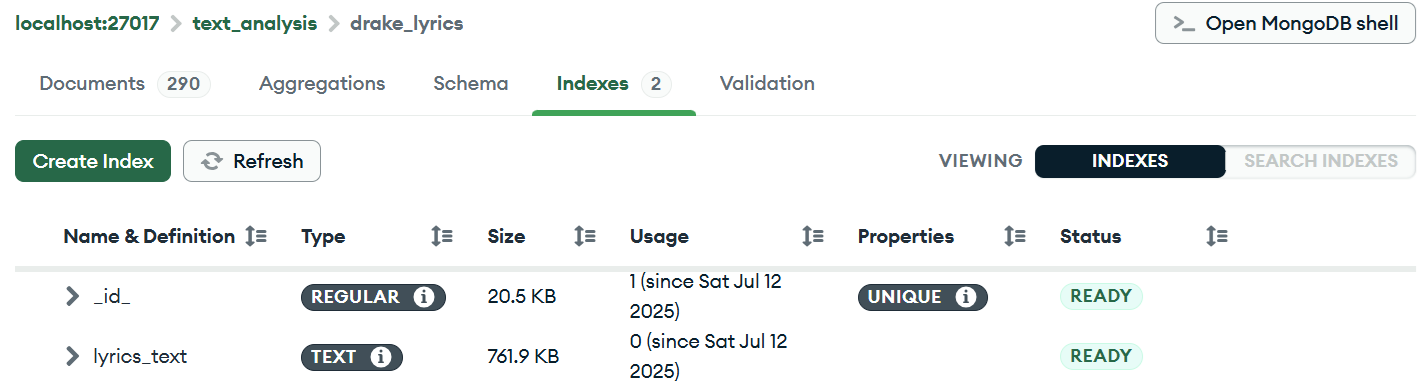
\includegraphics[width=0.8\textwidth]{./indices_drake.png}
    \caption{Índice de texto en lyrics}\label{fig:indicesdrake}
\end{figure}

\begin{figure}[H]
    \centering
    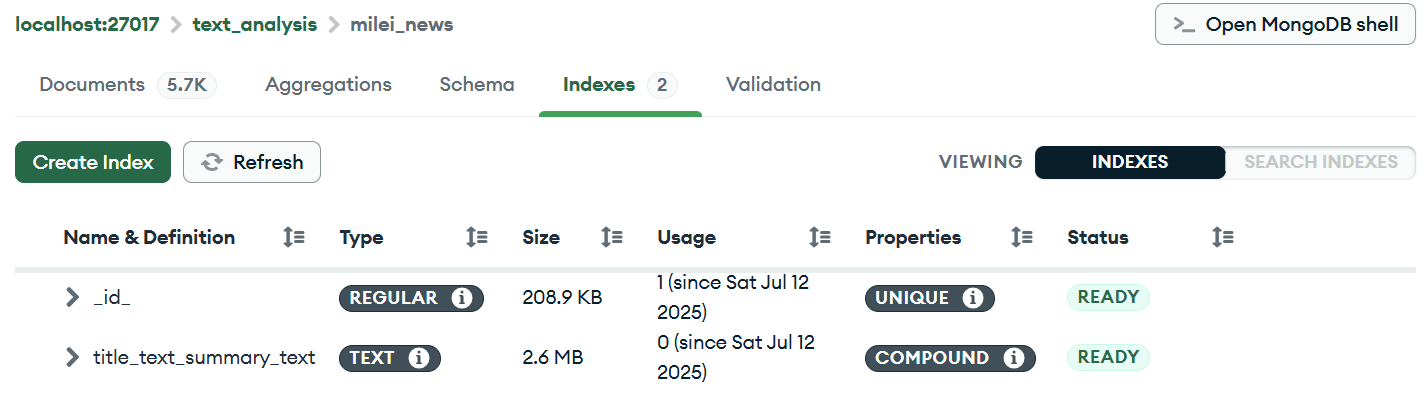
\includegraphics[width=0.8\textwidth]{./indices_milei.png}
    \caption{Índice de texto compuesto en title y summary}\label{fig:indicesmilei}
\end{figure}

\subsection{Consultas y Resultados}